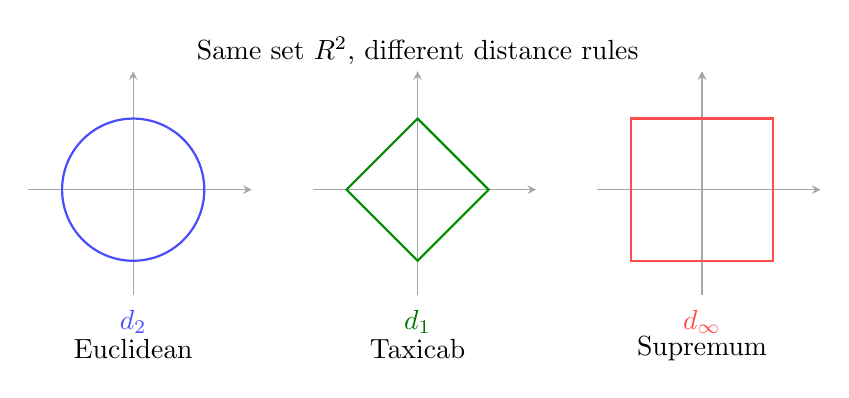
\begin{tikzpicture}[scale=0.86,>=stealth]
  \draw[->,gray!70] (-1.55,0) -- (1.75,0);
  \draw[->,gray!70] (0,-1.55) -- (0,1.75);
  \draw[blue!70,thick] (0,0) circle (1.05);
  \node[blue!70] at (0,-1.95) {\(d_2\)};
  \node at (0,-2.35) {Euclidean};

  \begin{scope}[xshift=4.2cm]
    \draw[->,gray!70] (-1.55,0) -- (1.75,0);
    \draw[->,gray!70] (0,-1.55) -- (0,1.75);
    \draw[green!55!black,thick]
      (0,1.05) -- (1.05,0) -- (0,-1.05) -- (-1.05,0) -- cycle;
    \node[green!45!black] at (0,-1.95) {\(d_1\)};
    \node at (0,-2.35) {Taxicab};
  \end{scope}

  \begin{scope}[xshift=8.4cm]
    \draw[->,gray!70] (-1.55,0) -- (1.75,0);
    \draw[->,gray!70] (0,-1.55) -- (0,1.75);
    \draw[red!70,thick] (-1.05,-1.05) rectangle (1.05,1.05);
    \node[red!70] at (0,-1.95) {\(d_\infty\)};
    \node at (0,-2.35) {Supremum};
  \end{scope}

  \node[align=center] at (4.2,2.05)
    {Same set \(\mathbb{R}^2\), different distance rules};
\end{tikzpicture}
